\newpage
\section{Agenti basati su conoscenza}
C'è bisogno di rappresentare la conoscenza in maniera parziale e incompleta (gli ambienti sono parzialmente osservabili). Ci servono quindi dei linguaggi più espressivi e con \textbf{capacità inferenziali}.\\
\subsection{Knowledge Base}
L'insieme di tutta la conoscenza necessaria a decidere un'azione da compiore è la \textbf{knowledge base} e può essere definita in due modi:
\begin{itemize}
	\item \textit{Dichiarativo}: all'agente viene detto cosa deve sapere, partendo da una conoscenza di base vuota e aggiungendo progressivamente formule (TELL)
	\item \textit{Procedurale}: si scrive un programma che definisca il processo decisionale una volta per tutte
\end{itemize}

\begin{definition}[Knowledge Base]
	Un insieme di \emph{enunciati} (formule) espressi in un linguaggio di rappresentazione.
\end{definition}

\begin{example}[Wumpus World]
	\label{example:wumpus_world}
	Il mondo del Wumpus è una caverna fatta di stanze connesse tra loro. All'interno c'è questa bestia puzzolente che mangia chiunque entri nella stanza in cui si trova. Questo può essere ucciso dall'agente che ha una freccia a disposizione.\\
	Ci sono delle stanze con degli \textit{ostacoli}: pozzi, in cui se l'agente entra, muore. In una delle stanze si trova l'\textit{obiettivo}, ovvero un lingotto d'oro.\\
	L'agente non conosce l'ambiente e la sua posizione, se non all'inizio.
	\begin{center}
		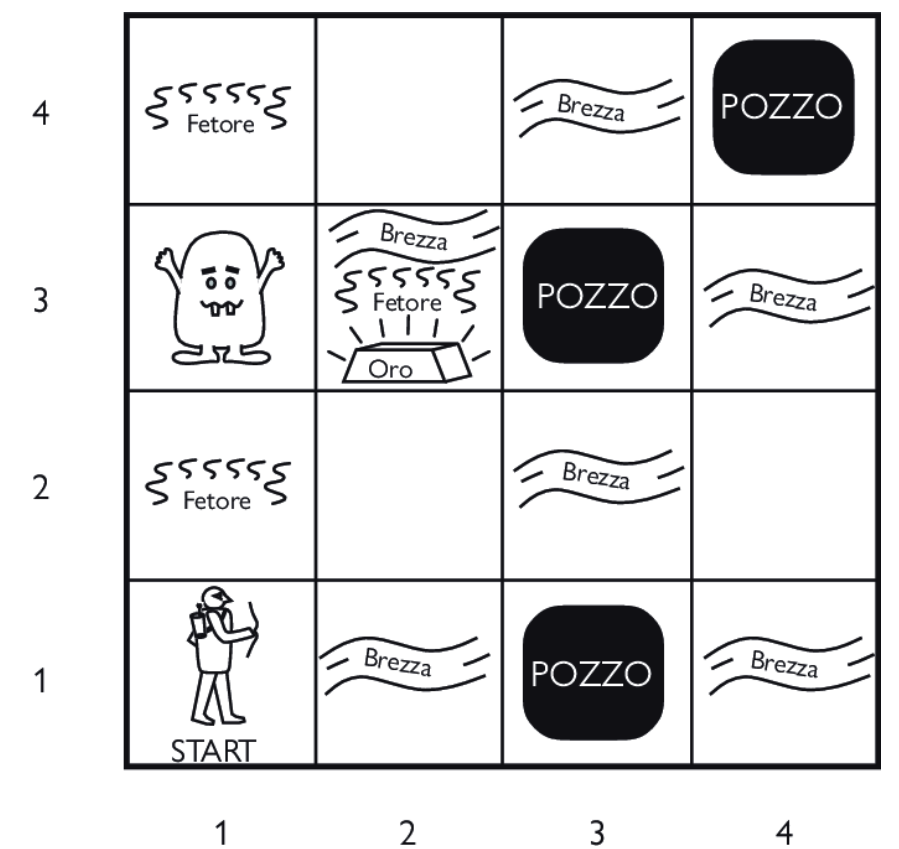
\includegraphics[scale=0.21]{wumpus_world.png}
	\end{center}
	Definiamo le \textbf{misure di prestazione}:
	\begin{itemize}
		\item +1000 se trova l'oro, torna in [1,1] ed esce
		\item -1000 se muore
		\item -1 per ogni azione
		\item -10 se usa la freccia
	\end{itemize}
	Invece l'\textbf{ambiente} è una griglia 4x4 circondata da pareti di delimitazione. L'agente inizia sempre nella posizione [1,1] rivolto verso destra (la prima casella è sempre safe). Le posizioni dell'oro e della bestia sono casuali e tutti i riquadri hanno una probabilità di $0.2$ di contenere un pozzo.\\
	L'agente può fare le seguenti \textbf{azioni}:
	\begin{itemize}
		\item Andare avanti
		\item Ruotare a destra o a sinistra di $90°$
		\item Afferrare un oggetto
		\item Scagliare la freccia
		\item Uscire
	\end{itemize}
	Il nostro agente puo \textbf{percepire} le seguenti cose:
	\begin{itemize}
		\item \textit{Fetore} nelle caselle adiacenti alla bestia
		\item \textit{Brezza} nelle caselle adiacenti ai pozzi
		\item \textit{Luccichio} nella casella con l'oro
		\item \textit{Urlo} se la bestia viene uccisa
	\end{itemize}
	e vengono rappresentati come una quintupla, che ad  esempio nella prima casella vale:
	\begin{equation*}
		[none,none,none,none,none]
	\end{equation*}
	Di conseguenza sappiamo che nelle caselle adiacenti non ci sono né pozzi né la bestia.
\end{example}

\subsubsection{Tell-Ask}
L'agente interagisce con la knowledge base tramite un'interfaccia funzionale di tipo Tell-Ask:
\begin{itemize}
	\item \textit{Tell}: aggiungere nuovi enunciati
	\item \textit{Ask}: interagire con la knowledge base
	\item \textit{Retract}: eliminirare enunciati
\end{itemize}
Gli enunciati nella KB rappresentano le credenze dell'agente e le risposte $\alpha$ devpomp essere tali per cui queste discendano necessariamente dalla KB.\\
Il problema fondamentale è quindi capire, data una base di conoscenza KB, come dedurre che un certo fatto $\alpha$ è vero di conseguenza.
\begin{equation}
	KB \models \alpha
\end{equation}
Un programma basilare è il seguente:
\begin{lstlisting}
	function Agente-KB (percezione) returns azione
		persistent: KB, una base di conoscenza
			t, un contatore, inizialmente a 0, che indica il tempo
		TELL(KB, Costruisci-Formula-Percezione(percezione, t ))
		azione = ASK(KB, Costruisci-Query-Azione( t ))
		TELL(KB, Costruisci-Formula-Azione(azione, t ))
		t = t + 1
		return azione
\end{lstlisting}
\subsubsection{Analisi}
A differenza di una \textit{base di dati}, la base di conoscenza non contiene solo fatti specifici da recuperare ma anche fatti generali, oregole, espressi in maniera esplicita in un linguaggio compatto. Questo le conferisce la \textbf{capacità inferenziale}, ovvero derivare nuovi fatti da quelli memorizzati.\\
Il lato negativo è che, avendo un linguaggi  più espressivo, è \textbf{meno efficiente} il meccanismo inferenziale. Serve quindi trovare il giusto bilanciamento da \textit{espressività} del linguaggio e \textit{complessità} del meccanismo inferenziale.

\subsection{Logica}
Le KB sono costituite da enunciati espresse secondo le regole della \textbf{sintassi}. La \textbf{semantica} invece ne esprime il significato. Un \textbf{modello} è una configurazione dei valori di verità che si possono assegnare alle variabili di una formula.
\subsubsection{Formalismo}
Un formalismo per la rappresentazione della conoscenza si compone di:
\begin{itemize}
	\item Una \textbf{sintassi}: un linguaggio composto da un vocabolario e da regole per la formulazione degli enunciati
	\item Una \textbf{semantica}: stabilisce una corrispondenza tra gli enunciati e ifatti del mondo
	\item Un \textbf{meccanismo inferenziale} che ci consente di inferire nuovi fatti
\end{itemize}
\begin{center}
	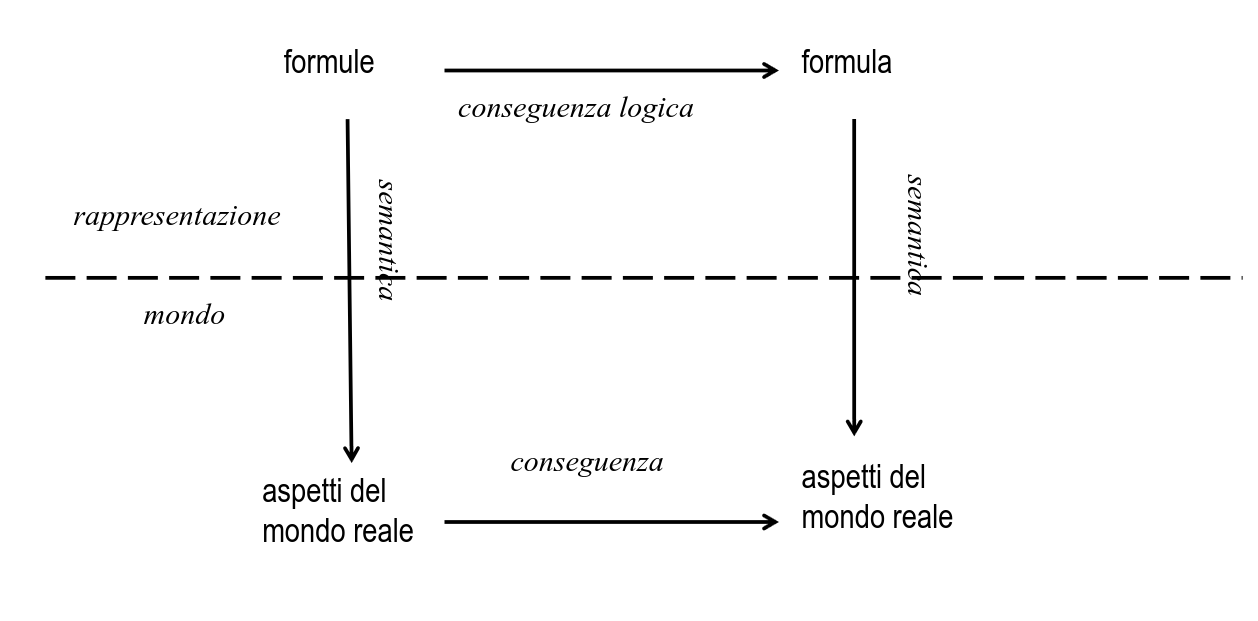
\includegraphics[scale=0.25]{formalismo.png}
\end{center}
Facendo il paragone con l'agente, le formule sono le sue configuraziini fisiche e il ragionamento è il processo di costruzione di nuove configurazioni a partire dalle vecchie. Il ragionamento logico deve assicurare che le nuove configurazioni siano effettive conseguenze sul mondo causate dalle vecchie configurazioni.

\section{Logica proposizionale}
\subsection{Sintassi}
La sintassi è la seguente, rappresentata in BNF:
\begin{equation}
	\begin{split}
		formula & \to formulaAtomica \vert formulaComplessa \\
		formulaAtomica & \to True \vert False \vert simbolo \\
		simbolo & \to P \vert Q \vert R \vert \ldots \\
		formulaComplessa & \to \neg formula \\
		&\vert (formula \land formula) \\
		& \vert (formula \lor formula)\\
		& \vert (formula \Rightarrow formula)\\
		& \vert (formula \Leftrightarrow formula)
	\end{split}
\end{equation}

\subsection{Semantica}
La logica proposizionale segue una semantica \textbf{composizionale}, dove il significato di una frase è determinato dal significato dei suoi componenti a partire dai \textit{simboli proposizionali}. Di seguito la ravola di verità:
\begin{table}[h!]
	\centering
	\begin{tabular}{|cc|ccccc|}
		\hline
		$P$ & $Q$ & $\neg P$ & $P \land Q$ & $P \lor Q$ & $ P \Rightarrow Q$ & $P \Leftrightarrow Q$\\
		\hline
		false & false & true & false & false & true & true \\
		false & true & true & false & true & true & false \\
		true & false & false & false & true & false & false \\
		true & true & false & true & true & true & true\\
		\hline
	\end{tabular}
\end{table}

\subsection{Conseguenza logica}
\begin{definition}[Conseguenza logica]
	Una formula $\alpha$ è una conseguenza logica di un insieme di formule KB se e solo se in ogni modello di KB, anche $\alpha$ è vera ($KB \models \alpha$).
\end{definition}
Indichiamo con $M(KB)$ i modelli dell'insieme di formule in KB e con $M(\alpha)$ l'insieme delle interpretazioni che rendono $\alpha$ vera, ovvero i suoi \textbf{modelli}.
\begin{equation}
	KB \models \alpha \Leftrightarrow M(KB) \subseteq M(\alpha)
\end{equation}

\subsubsection{Model checking}
Un modo per determinare la conseguenza logica è quello di enumere i \textit{modelli} e mostrare che la formula $\alpha$ vale in tutti quelli in cui è vera la KB.

\begin{example}[Wumpus World]
	Partendo dall'esempio \ref{example:wumpus_world} abbiamo che la KB iniziale, $KB_0$, è costituita dalle regole descritte nella definizione dell'esercizio:
		\begin{gather*}
			\neg W_{1,1} \quad \neg P_{1,1} \\
			B_{2,1} \Leftrightarrow (P_{1,1} \lor P_{2,2,} \lor P_{3,1})\\
			B_{1,1} \Leftrightarrow (P_{1,2} \lor P_{2,1})\\
			\vdots
		\end{gather*}
		Il primo passo dell'agente è spostarsi in $[2,1]$ dato che in $[1,1]$ non ha percepito niente. Abbiamno quindi:
		\begin{equation*}
			KB_1 = KB_0 \cup \{\neg B_{1,1}, B_{2,1}, \neg F_{1,1}, \neg F_{2,1}, \ldots\}
		\end{equation*}
		e rappresentiamo le domande sulla presenza o meno di pozzi come:
		\begin{equation*}
			\begin{split}
				KB_1 \models \neg P_{1,2} \\
				KB_1 \models \neg P_{2,2} \\
				KB_1 \models \neg P_{3,1} \\
			\end{split}
		\end{equation*}
		Sapendo da $KB_0$ che non ci sono pozzi nella casella $[1,1]$ e che c'è un pozzo nella stanza adiacente solo se ci percepisce la brezza, formuliamo le seguenti proposizioni:
		\begin{equation*}
			\begin{split}
				& B_{1,1} \Leftrightarrow (P_{1,2} \lor P_{2,1}) \\
				& B_{2,1} \Leftrightarrow (P_{1,1} \lor P_{2,2} \lor P_{3,1})
			\end{split}
		\end{equation*}
		e concludiamo che non c'è brezza in $[1,1]$ e c'è in $[2,1]$, ovvero $\neg B_{1,1}$ e $B_{2,1}$.\\
		Ci rimangono quindi tre configurazioni possibili dato che abbiamo:
		\begin{gather*}
			KB_1 \models \neg P_{1,2}\\
			KB_1 \models P_{2,2}\lor P_{3,1}
		\end{gather*}
		e sono quelle in cui i pozzi sono in $[3,1]$ oppure in $[2,2]$ oppure in entrambi.i
\end{example}

\subsubsection{SAT}
Un altro approccio alla dimostrazione della conseguenza logica si basa su tre principi:
\begin{itemize}
	\item \textbf{Equivalenza logica}: due formule $\alpha$ e $\beta$sono equivalenti se sono vere nello stesso insieme di modelli
	\begin{equation}
		\alpha \equiv \beta \Leftrightarrow \alpha \models \beta\land\beta\models\alpha
	\end{equation}
	Alcune leggi fondamentali per l'equivalenza sono:
	\begin{itemize}
		\item \textit{Commutatività}: $(\alpha\land\beta)\equiv(\beta\land\alpha)\quad(\alpha\lor\beta)\equiv(\beta\lor\alpha)$
		\item \textit{Associatività}: $((\alpha\land\beta)\land\gamma)\equiv(\alpha\land(\beta\land\gamma))\quad((\alpha\lor\beta)\lor\gamma)\equiv(\alpha\lor(\beta\lor\gamma))$
		\item \textit{Eliminazione della doppia negazione}: $\neg(\neg\alpha)$
		\item \textit{Contrapposizione}: $(\alpha\Rightarrow\beta)\equiv(\neg\beta\Rightarrow\neg\alpha)$
		\item \textit{Eliminazione dell'implicazione}: $(\alpha\Rightarrow\beta)\equiv(\neg\alpha\lor\beta)$
		\item \textit{Eliminazione del bicondizionale}: $(\alpha\Leftrightarrow\beta)\equiv((\alpha\Rightarrow\beta)\land(\beta\Rightarrow\alpha))$
		\item \textit{De Morgan}: $\neg(\alpha \land\beta)\equiv(\neg\alpha\lor\neg\beta)\quad\neg(\alpha \lor\beta)\equiv(\neg\alpha\land\neg\beta)$
		\item \textit{Distributività}: $(\alpha\land(\beta\lor\gamma))\equiv((\alpha\land\beta)\lor(\alpha\land\gamma)\quad(\alpha\lor(\beta\land\gamma))\equiv((\alpha\lor\beta)\land(\alpha\lor\gamma))$
	\end{itemize}
	\item \textbf{Validità}: una formula $\alpha$ è valida se e solo se è vera in tutte le sue interpretazioni. In quel caso sono anche dette \textbf{tatutologie}.
	\begin{theorem}[Teorema di deduzione e refutazione]
		Date due formule $\alpha$ e $\beta$, allora $\alpha \models\beta \Leftrightarrow (\alpha\Rightarrow\beta)$. Possiamo riscriverlo, usando le leggi appena elencate, anche come $\alpha\models\beta \Leftrightarrow (\alpha \land \neg\beta)$, che ci permette di fare la dimostrazione per \textbf{assurdo}.
	\end{theorem}
	\item \textbf{Soddisfacibilità}: una formula $\alpha$ è soddisfacibile se e solo se esiste una interpretazione in cui $\alpha$ è vera (ovvero se esiste un modello di $\alpha$). La determinazione della soddisfacibilità è il problema \textbf{SAT}.
\end{itemize}
Si noti che \textit{validità} e \textit{soddisfacibilità} sono connesse:
\begin{itemize}
	\item $\alpha$ è valida se e solo se $\neg\alpha$ è insoddisfacibile
	\item $\alpha$ è soddisfacibvile se e solo se $\neg\alpha$ non è valida
\end{itemize}
\begin{definition}[Forma a clausole]
	La forma a clausole è la \textbf{forma normale congiuntiva} (CNF), ovvero una congiunzione di disgiunzioni di letterali (un simbolo o la sua negazione). È sempre possibile ottenerla con trasformazioni che preservano l'equivalenza logica.
\end{definition}
Per eseguire una trasformazione in forma a clausole bisogna seguire i seguenti passi:
\begin{enumerate}
	\item Eliminazione del $\Leftrightarrow$
	\item Eliminazione del $\Rightarrow$
	\item Portare le negazioni all'interno tramite De Morgan
	\item Distribuire $\lor$ su $\land$
\end{enumerate}

\begin{example}
	Partendo dall'esempio \ref{example:wumpus_world}, trasformiamo $B_{1,1} \Leftrightarrow (P_{1,2}\lor P_{2,1})$:
	\begin{enumerate}
		\item $(B_{1,1} \Rightarrow (P_{1,2} \lor P_{2,1})) \land ((P_{1,2} \lor P_{2,1}) \Rightarrow B_{1,1})$
		\item $(\neg B_{1,1} \lor (P_{1,2} \lor P_{2,1})) \land (\neg(P_{1,2} \lor P_{2,1}) \lor B_{1,1})$
		\item $(\neg B_{1,1} \lor (P_{1,2} \lor P_{2,1})) \land ((\neg P_{1,2} \land \neg P_{2,1}) \lor B_{1,1})$
		\item $(\neg B_{1,1} \lor P_{1,2} \lor P_{2,1}) \land (\neg(P_{1,2} \lor B_{1,1}) \land (\neg P_{2,1} \lor B_{1,1})$
	\end{enumerate}
	che possiamo riscrivere come
	\begin{equation*}
		\{\neg B_{1,1}, P_{1,2}, P_{2,1}\}\{\neg P_{1,2}, B_{1,1,}\}\{\neg P_{2,1}, B_{1,1}\}
	\end{equation*}
\end{example}

\newpage
\subsection{Algoritmi}
Di seguito alcuni algoritmi per determinare se è vera una conseguenza logica a partire da una KB.
\subsubsection{TV-Consegue}
Questo algoritmo enumera tutte le possibili interpretazioni di KB, e per ciascuna interpretazione se soddisfa la KB controlla che soddisfi anche $\alpha$. Basta trovare una singola interpretazione che soddisfa la KB ma non $\alpha$ per determinare una risposta negativa. Avremo quindi, dati $k$ simboli, $2^k$ possibili interpretazioni.
\label{alg:tv_consegue}
\begin{lstlisting}
	function TV-Consegue?(KB, a) // Restituisce true oppure false
		inputs: KB, la base di conoscenza, una formula della logica proposizionale
			a, la query, una formula della logica proposizionale
	simboli = una lista dei simboli proposizionali contenuti in KB e a
	return TV-Verifica-Tutto(KB, a, simboli, { })
	
	function TV-Verifica-Tutto(KB, a, simboli, modello) // Restituisce true oppure false
		if Vuoto?(simboli) then
			if PL-Vero?(KB, modello) then return PL-Vero?(a, modello)
			else return true // Quando KB false, restituisce sempre true
		else do
			P = Primo(simboli); resto = Resto(simboli)
			return TV-Verifica-Tutto(KB, a, resto, modello = {P = true})
					  and
					  TV-Verifica-Tutto(KB, a, resto, modello = {P = false})
\end{lstlisting}

\begin{example}
	Supponiamo di voler verificare la seguente conseguenza logica:
	\begin{equation*}
		(\neg a\lor b)\land(a \lor c) \models (b \lor c)
	\end{equation*}
	Ci costruiamo la tabella di verità:
	\begin{table}[!h]
		\centering
		\begin{tabular}{|ccc|cc|}
			\hline
			$a$&$b$&$c$&$\neg a \lor b$ & $a \lor c$ \\
			\hline
			T & T & T & T & T\\
			T & T& F & T & T \\
			T & F &T&F&T\\
			T&F&F&F&T\\
			F&T&T&T&T\\
			F&T&F&T&F\\
			F&F&T&T&T\\
			F&F&F&T&F\\
			\hline
		\end{tabular}
	\end{table}
	Per poi selezionare solo le righe in cui la KB è vera e verificare se la nostra formula è sempre vera:
	\begin{table}[!h]
		\centering
		\begin{tabular}{|ccc|cc|c|}
			\hline
			$a$&$b$&$c$&$\neg a \lor b$ & $a \lor c$ & $b\lor c$\\
			\hline
			T & T & T & T & T & T\\
			T & T& F & T & T & T\\
			F&T&T&T&T & T\\
			F&F&T&T&T&T\\
			\hline
		\end{tabular}
	\end{table}
	Quindi la risposta è sì.\\
	Applicando l'algoritmo \ref{alg:tv_consegue} abbiamo la seguente esecuzione:
	\begin{lstlisting}
		TV-VERIFICA-TUTTO(KB, formula, [a, b, c], { })
			TV-VERIFICA-TUTTO(KB, formula, [b, c], {a=T})
				TV-VERIFICA-TUTTO(KB, formula, [c], {a=T, b=T})
					TV-VERIFICA-TUTTO(KB, formula, [ ], {a=T, b=T, c=T}) // OK
					TV-VERIFICA-TUTTO(KB, formula, [ ], {a=T, b=T, c=F}) // OK
				TV-VERIFICA-TUTTO(KB, formula, [c], {a=T, b=F})
					TV-VERIFICA-TUTTO(KB, formula, [ ], {a=T, b=F, c=T}) // OK
					TV-VERIFICA-TUTTO(KB, formula, [ ], {a=T, b=F, c=F}) // OK
			TV-VERIFICA-TUTTO(KB, formula, [b, c], [a=F])
			etc...
	\end{lstlisting}
\end{example}
\subsubsection{DPLL}
Questo algoritmo parte da una KB in forma a clausole e prende in input una formula in CNF ed enumera ricorsivamente in profondità tutte le possibili interpretazioni alla ricerca di un modello. Per avere un miglioramento sull'algoritmo \ref{alg:tv_consegue} applico tre clausole:
\begin{itemize}
	\item \textbf{Terminazione anticipata}: si può decidere sulla verità di una clausola anche con interpretazioni parziali, ovvero quando ho degli \textit{OR} basta che un simbolo sia vero mentre quando ho degli \textit{AND} basta che unpo sia falso per rendere falsa l'intera interpretazione
	\item \textbf{Euristica dei simboli puri}: un simbolo puro è un simbolo che appare con lo stesso segno in tutte le clausole (trascurando eventualmente quelle già rese vere). Possono poi essere assegnati a True se il letterale è positivo o a False se è negativo
	\item \textbf{Euristica delle clausole unitarie}: una clausola in cui è rimasto un solo letterale non assegnato
\end{itemize}

\begin{lstlisting}
	function DPLL-Soddisfacibile?(s) returns true oppure false
			inputs: s, una formula della logica proposizionale
		clausole = insieme di clausole nella rappresentazione CNF di s
		simboli = una lista di tutti i simboli proposizionali in s
		return DPLL(clausole, simboli, { })
	
	function DPLL(clausole, simboli, modello) returns true oppure false
		if ogni clausola in clausole vera in modello then return true
		if qualche clausola in clausole falsa in modello then return false
		P, valore = Trova-Simbolo-Puro(simboli, clausole, modello)
		if P diverso da null then return DPLL(clausole, simboli - P, modello = {P = valore})
		P, valore = Trova-Clausola-Unitaria(clausole, modello)
		if P diverso da null then return DPLL(clausole, simboli-P, modello = {P = valore})
		P = Primo(simboli); resto = Resto(simboli)
		return	DPLL(clausole, resto, modello = {P = true})
					 or
					 DPLL(clausole, resto, modello = {P = false})
\end{lstlisting}

\begin{example}
	Supponiamo di voler verificare la seguente conseguenza logica:
	\begin{equation*}
		\{\neg B_{1,1}, P_{1,2}, P_{2,1}\}\{\neg P_{1,2}, B_{1,1}\}\{\neg P_{2,1}, B_{1,1}\}\{\neg B_{1,1}\} \models \{\neg P_{1,2}\}
	\end{equation*}
	Aggiungiamo alla KB la clausola $\{P_{1,2}\}$ e verifichiamo con SAT se l'insieme è insoddisfacibile:
	\begin{enumerate}
		\item La clausola $\{P_{1,2}\}$ è unitaria, quindi $P_{1,2}=True$. Di conseguenza $\{\neg B_{1,1}, P_{1,2}, P_{2,1}\}$ e $\{P_{1,2}\}$ sono soddisfatte e rimaniamo con
		\begin{equation*}
			\{\neg P_{1,2}, B_{1,1}\}\{\neg P_{2,1}, B_{1,1}\}\{\neg B_{1,1}\}
		\end{equation*}
		\item $P_{2,1}$ è un simbolo puro ed essendo negativo sarà uguale a False, quindi la clausola $\{\neg P_{2,1}, B_{1,1}\}$ è soddisfatta e rimaniamo con
		\begin{equation*}
			\{\neg P_{1,2}, B_{1,1}\}\{\neg B_{1,1}\}
		\end{equation*}
	\end{enumerate}
	Dato che non esistono modelli possiamo dire che $\neg P_{1,2}$ è conseguenza logica della KB
\end{example}
Questo algoritmo è \textbf{completo} e \textbf{termina sempre}. Alcuni miglioramenti sono:
\begin{itemize}
	\item Se possibile scomporre in sotto problemi indipendenti (quando non hanno simboli in comune)
	\item Ordinare le variabili per frequenza di comparizione
	\item Backtracing intelligente
\end{itemize}